\chapter{Law of Reflection}

\section{Aim}
To discover the relationship between the incident angle and reflected angle of a plane mirror

\section{Background Information}
Nearly every object can be seen because light reflects off of its surface and then enters your eye. Reflection is when light rays bounce off the surface of an object. Drivers use sight mirrors to observe cars behind them, in saloons there are shaving mirrors, and mirrors have many other applications in industry and science. What is the relationship between the incident angle and reflected angle of a plane mirror? 

\section{Materials}
Plane mirror, 4 optical pins, soft board, 4 drawing pins, mirror, ruler, 2 plain papers, graph paper, pencil and protractor

\section{Procedure}
\begin{enumerate}
\item Pin a piece of paper onto the middle of a soft board.
\item Draw a line MM’ of 15 cm in the middle of the paper.  
\item Draw a perpendicular line on the midpoint of MM’ and call it ON as seen in Figure \ref{fig:law-of-reflection-1}. This line is called a normal line.
\item Draw a line AO making an angle of incidence $i$ from the normal.  
\item Place a plane mirror vertically on the line MM’.
\item Insert two pins P$_1$ and P$_2$ on the line AO.
\item Look from the opposite side of the normal at the images of the pins P$_1$ and P$_2$ in the mirror. Insert two other pins, P$_3$ and P$_4$, so that they appear to be in a straight line with the images of P$_1$ and P$_2$ in the mirror.
\item Remove the pins and draw lines through the marks of the pins up to the line MM’.
\item Using a protractor measure and record the angle of incidence, $i$, and the angle of reflection, $r$, both taken with respect to the normal ON. 
\item Repeat the experiment by varying the angle of incidence, $i$, to obtain four more values of $r$. Tabulate the results.
\item Observe which planes the incident ray, reflected ray and the normal line occur in. 
\end{enumerate}

\begin{figure}[h!]
\centering
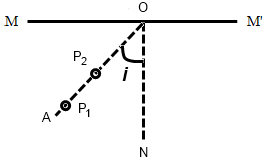
\includegraphics[width=8cm]{./img/law-of-reflection-1.png}
\caption{Law of Reflection practical setup}
\label{fig:law-of-reflection-1}
\end{figure}

\section{Analysis and Interpretation}
\begin{enumerate}
\item Draw a graph of incident angle $i$ against reflected angle $r$.
\item From the graph determine the slope.
\end{enumerate}

\section{Conclusion}
\begin{enumerate}
\item What is the relationship between the incident angle and reflected angle of a plane mirror?
\item From the experiment do the incident ray, reflected ray and normal all occur in one plane? 
\end{enumerate}

\section{Questions for Discussion}
\begin{enumerate}
\item What will happen if the mirror is not silvered on one side?
\item What are the sources of error in this experiment?
\item Why where two optical pins used to construct each line instead of only one?
\item If the object is placed 20$^\circ$ from the normal, will the image be observed at a reflected angle of 40$^\circ$?
\item What could be used instead of optical pins in this experiment?
\end{enumerate}

\section{Reflection and Self Assessment}
\begin{enumerate}
\item Was the experiment helpful to you? Explain.
\item What are some of the challenges you encountered in the experiment? Suggest ways to overcome them.
\item Where can the results of this experiment be applied in your daily life? 
\end{enumerate}